\documentclass[12pt, letterpaper]{article}

% --- PAQUETES DE IDIOMA Y FORMATO ---
\usepackage[utf8]{inputenc}
\usepackage[spanish]{babel}
\usepackage[margin=2.5cm]{geometry}
\usepackage{graphicx} 
\usepackage{hyperref} 
\usepackage{xcolor}   
\usepackage{listings}
\usepackage{booktabs} 
\usepackage{float}

% --- CONFIGURACIÓN PARA EL CÓDIGO C++ ---
\definecolor{codegreen}{rgb}{0,0.6,0}
\definecolor{codegray}{rgb}{0.5,0.5,0.5}
\definecolor{codepurple}{rgb}{0.58,0,0.82}
\definecolor{backcolour}{rgb}{0.95,0.95,0.92}

\lstdefinestyle{mystyle}{
	backgroundcolor=\color{backcolour},   
	commentstyle=\color{codegreen},
	keywordstyle=\color{magenta},
	numberstyle=\tiny\color{codegray},
	stringstyle=\color{codepurple},
	basicstyle=\ttfamily\footnotesize,
	breakatwhitespace=false,         
	breaklines=true,                 
	captionpos=b,                    
	keepspaces=true,                 
	numbers=left,                    
	numbersep=5pt,                  
	showspaces=false,                
	showstringspaces=false,
	showtabs=false,                  
	tabsize=2
}
\lstset{style=mystyle}

% --- INICIO DEL DOCUMENTO ---
\begin{document}
	
	% --- PORTADA ---
	\begin{titlepage}
		\centering
		\vspace*{0.5cm}
		
		% Logotipos (Asegúrate de incluir 'logo_motorsport.png' en tu directorio)
		
\includegraphics[width=2.8cm]{logo_unam.png} 
		\hfill
		
\includegraphics[width=3.2cm]{logo_motorsport.png}
		\hfill
		
\includegraphics[width=2.8cm]{logo_fi.png} 
		\\[1cm] 
		
		{\Huge \textbf{Universidad Nacional Autónoma de México}}\\[0.5cm]
		{\LARGE \textbf{Facultad de Ingeniería}}\\[1cm]
		
		{\Large Proceso de Reclutamiento Agrupación: UNAM Motorsports — División de Data Acquisition}\\[0.5cm]
		{\Large Proyecto: Sistema de Validación de Plausibilidad del APPS (Accelerator Pedal Position Sensor)}\\[1cm]
		
		% Título del Reporte
		\rule{\linewidth}{0.5mm} \\[0.4cm]
		{ \huge \bfseries Reporte Técnico Final: \\ Análisis, Diseño e Implementación de un Sistema de Seguridad Embebido para Sensor de Posición del Pedal de Aceleración (APPS) }\\[0.4cm]
		\rule{\linewidth}{0.5mm} \\[1.5cm] 
		
		\begin{flushleft}
			\Large \textbf{Autor:}\\
			\vspace{0.3cm}
			\normalsize
			$\bullet$ Francisco José Coutiño Morales (Núm. Cta: 425121623)\\ 
		\end{flushleft}
		
		\vfill 
		
		{\large \today} 
	\end{titlepage}
	
	% --- ÍNDICE ---
	\newpage
	\tableofcontents
	\newpage
	
	% =========================================================================
	% --- SECCIÓN 1: INTRODUCCIÓN ---
	% =========================================================================
	\section{Introducción}
	El presente documento detalla el análisis, el diseño electrónico, la arquitectura de software y el proceso de depuración llevado a cabo para el desarrollo de la Actividad 1 del proceso de reclutamiento de UNAM Motorsport: un sistema de validación de plausibilidad para el Sensor de Posición del Pedal del Acelerador (APPS, por sus siglas en inglés), implementado sobre un microcontrolador ESP32 y fundamentado en el marco normativo de Formula SAE.
	
	El objetivo central de esta actividad no es únicamente leer la posición de un pedal, sino construir un \textbf{sistema de seguridad crítico}: un mecanismo capaz de detectar, con tiempos de respuesta acotados y de forma determinista, cuándo la información que recibe de sus sensores deja de ser confiable, y de actuar en consecuencia cortando la habilitación del motor antes de que dicha falla pueda traducirse en una aceleración no intencionada del vehículo.
	
	\subsection{Contexto Normativo: Formula SAE y la Regla T.4.2}
	En un vehículo de Formula SAE real, el pedal del acelerador no está conectado mecánicamente al cuerpo de aceleración (throttle body); la señal viaja de forma electrónica desde el pedal hasta la ECU (Electronic Control Unit), la cual decide cuánta potencia entregar al motor. A este esquema se le conoce como \textit{drive-by-wire}. La consecuencia directa de eliminar el enlace mecánico es que, si el sensor que reporta la posición del pedal falla o entrega una lectura errónea, el vehículo podría interpretar que el piloto está pisando el acelerador cuando en realidad no lo está haciendo, generando una condición de aceleración involuntaria (\textit{Unintended Acceleration}), uno de los riesgos de seguridad más graves que puede presentar un vehículo de competencia.
	
	Por esta razón, el reglamento de Formula SAE, en su sección T.4 (relativa al sistema de control del acelerador), exige explícitamente el uso de \textbf{dos sensores redundantes e independientes} para medir la posición del pedal, junto con lógica de supervisión (\textit{plausibility check}) que compare ambas lecturas de forma continua. Si la diferencia entre ambos canales excede un umbral definido durante un tiempo sostenido, el sistema debe cortar la potencia del motor de forma inmediata. Este es, precisamente, el problema de ingeniería que la presente actividad busca replicar a escala de prototipo, y es el criterio que guio cada decisión de diseño documentada en este reporte.
	
	\subsection{Flujo de Trabajo y Metodología de Desarrollo}
	El desarrollo del sistema siguió un enfoque iterativo, dividido en las siguientes fases:
	\begin{enumerate}
		\item \textbf{Fase de diseño conceptual}: definición de la arquitectura de tres capas (adquisición, calibración, seguridad), selección del microcontrolador (ESP32 DevKit V1) y planteamiento teórico del circuito de sensado mediante divisores de voltaje resistivos.
		\item \textbf{Fase de simulación}: construcción de un circuito virtual en Wokwi como primera validación del esquema eléctrico y del código antes de exponer hardware real a posibles errores de cableado.
		\item \textbf{Fase de implementación física}: armado del circuito sobre protoboard, carga del firmware al ESP32 mediante Arduino IDE, y validación en campo mediante el Monitor Serie.
		\item \textbf{Fase de depuración}: identificación y corrección sistemática de fallas de hardware (conexiones flojas, lecturas flotantes, desviaciones de calibración), descrita a detalle en la Sección 6 de este documento.
		\item \textbf{Fase de pruebas de validación}: ejecución de un protocolo de pruebas funcionales que confirma el comportamiento del sistema ante los escenarios de operación normal, falla real y ruido transitorio.
	\end{enumerate}
	
	% =========================================================================
	% --- SECCIÓN 2: FUNDAMENTO FÍSICO ---
	% =========================================================================
	\section{Fundamento Físico: El APPS en un Vehículo de Competencia Real}
	Para justificar cada decisión tomada en este proyecto es necesario entender la analogía directa entre el prototipo construido y el sistema real de un monoplaza de Formula SAE:
	
	\begin{itemize}
		\item \textbf{El pedal físico del piloto} se modela en este prototipo mediante \textbf{dos potenciómetros mecánicamente acoplados}. En un vehículo real, ambos sensores están montados sobre el mismo eje del pedal, de forma que cualquier movimiento del piloto mueve ambos sensores de manera simultánea y proporcional. En el prototipo, esta condición se simula girando ambas perillas al mismo tiempo y a la misma velocidad; desincronizar una perilla de la otra equivale a simular la falla mecánica o eléctrica de uno de los dos sensores.
		\item \textbf{Los divisores de voltaje resistivos} desempeñan el papel del acondicionamiento de señal que en un vehículo real realiza el arnés de sensores del APPS, adaptando el voltaje de salida del sensor al rango de entrada seguro del conversor analógico-digital (ADC) de la ECU.
		\item \textbf{La ECU real} se modela mediante el ESP32, que ejecuta el algoritmo de plausibilidad y decide si habilita o inhibe la señal de aceleración.
		\item \textbf{El corte del motor} se representa mediante el LED rojo de alerta y el pin \texttt{PIN\_SENAL\_INTERRUPCION}, el cual, en una implementación real, estaría conectado a la línea de corte de encendido/inyección o a un relevador de seguridad (\textit{kill switch} electrónico) en serie con el sistema de combustible o de ignición.
	\end{itemize}
	
	Esta analogía no es un detalle decorativo: es el criterio que define qué comportamientos del sistema son aceptables. Por ejemplo, la razón por la cual el sistema \textbf{no debe} activar una falla ante una discrepancia momentánea de un solo ciclo de muestreo es que, en pista, el ruido eléctrico y las vibraciones del vehículo pueden inducir picos de lectura de milisegundos que no representan una falla real del sensor; cortar el motor ante cada uno de esos picos haría el vehículo inmanejable. De ahí se deriva directamente la necesidad del filtro de \textit{debounce} de 100 ms implementado en la capa de seguridad.
	
	% =========================================================================
	% --- SECCIÓN 3: ARQUITECTURA DEL SISTEMA ---
	% =========================================================================
	\section{Arquitectura del Sistema: Diseño en Tres Capas Independientes}
	El firmware fue diseñado deliberadamente bajo un principio de \textbf{separación de responsabilidades}, análogo al Principio de Responsabilidad Única (SRP) aplicado a sistemas embebidos: cada capa del sistema tiene una única razón para cambiar, y ninguna capa conoce los detalles internos de la capa contigua más allá de la interfaz que consume.
	
	\subsection{Capa de Adquisición}
	Es la responsable exclusiva de obtener el voltaje crudo presente en cada canal del sensor, sin realizar ningún tipo de interpretación sobre ese valor. Se ejecuta bajo un temporizador de hardware a 1 kHz (una lectura cada 1 milisegundo), independiente del resto de la lógica del programa. Esta capa nunca decide si hay una falla; solo entrega datos.
	
	\subsection{Capa de Calibración}
	Traduce el valor crudo del ADC (un entero de 12 bits, en el rango 0--4095) a un porcentaje normalizado de 0 \% a 100 \%, que representa la posición real del pedal en una escala común y comprensible, independientemente de las particularidades eléctricas de cada canal. Esta capa es completamente independiente de la lógica de seguridad: si en el futuro se sustituyen las resistencias del divisor de voltaje, \textbf{únicamente es necesario modificar las cuatro constantes de calibración}, sin tocar ninguna línea de la lógica de decisión de falla.
	
	\subsection{Capa de Seguridad}
	Es el núcleo crítico del sistema. Toma los dos porcentajes ya normalizados —nunca los valores crudos del ADC— y determina si ambos canales son \textit{plausibles} entre sí, es decir, si su diferencia se mantiene dentro de un margen tolerable. Implementa, además, el filtro de \textit{debounce} de 100 ms que evita que ruido transitorio dispare un corte de motor innecesario, y gestiona la máquina de estados que determina si el sistema se encuentra en operación normal, en un estado transitorio de sospecha de falla, o en falla confirmada.
	
	Esta estratificación permite, entre otras cosas, que la capa de seguridad pueda ser certificada y auditada de forma aislada del resto del sistema —una práctica estándar en el desarrollo de software de seguridad crítica (\textit{safety-critical software}) en la industria automotriz— ya que su comportamiento depende únicamente de los porcentajes de entrada y de dos constantes (\texttt{UMBRAL\_PLAUSIBILIDAD\_PCT} y \texttt{TIEMPO\_DEBOUNCE\_MS}), y no de ningún detalle de la implementación eléctrica subyacente.
	
	% =========================================================================
	% --- SECCIÓN 4: DISEÑO ELECTRÓNICO ---
	% =========================================================================
	\section{Diseño Electrónico del Circuito}
	
	\subsection{Justificación del Divisor de Voltaje Asimétrico}
	Una de las decisiones de diseño más relevantes de este proyecto fue construir los dos canales de sensado con \textbf{rangos de voltaje distintos entre sí}, en lugar de utilizar dos divisores idénticos. El Canal 1 (conectado a \texttt{GPIO35}) se construyó con un divisor de 10 k$\Omega$ / 20 k$\Omega$, que produce un voltaje máximo teórico cercano a 3.3 V; el Canal 2 (conectado a \texttt{GPIO34}) se construyó con un divisor de 10 k$\Omega$ / 10 k$\Omega$, que produce un voltaje máximo teórico cercano a 2.5 V.
	
	\textbf{Justificación técnica:} esta asimetría no es un error de diseño, sino una decisión intencional que mejora la capacidad de diagnóstico del sistema. Si ambos canales compartieran exactamente el mismo rango eléctrico, un corto circuito a la línea de alimentación (5 V) o a tierra (GND) en cualquiera de los dos canales podría, en ciertos escenarios, producir lecturas que —una vez calibradas a porcentaje— coincidieran accidentalmente entre sí, enmascarando una falla real. Al forzar que cada canal tenga un tope eléctrico distinto, cualquier corto circuito hacia los rieles de alimentación empuja la lectura fuera del rango de calibración esperado para ese canal específico, generando una discrepancia porcentual detectable por la capa de seguridad. Este principio reproduce, a pequeña escala, una práctica real de la industria: la redundancia heterogénea de sensores mejora la observabilidad de fallas eléctricas frente a la redundancia homogénea.
	
	Es importante señalar que, durante el ensamblado físico, el potenciómetro con el divisor de mayor rango (10 k$\Omega$ / 20 k$\Omega$) terminó ubicado físicamente en la posición correspondiente a \texttt{D35} en lugar de \texttt{D34} como se había planteado en el diseño teórico inicial. Este desajuste se resolvió a nivel de software, intercambiando la asignación de \texttt{PIN\_SENSOR\_1} y \texttt{PIN\_SENSOR\_2} en el código, sin necesidad de rehacer el cableado físico — una muestra práctica de cómo el desacoplamiento entre hardware y firmware, propio de la capa de calibración descrita en la Sección 3.2, facilita este tipo de ajustes sin comprometer la arquitectura general del sistema.
	
	\subsection{Selección de Componentes y Distribución en Protoboard}
	El circuito físico final está compuesto por:
	\begin{itemize}
		\item 1 ESP32 DevKit V1 (30 pines), montado a horcajadas sobre el canal central de la protoboard para exponer ambas columnas de pines.
		\item 2 potenciómetros lineales de 10 k$\Omega$ (B10K), cuyo eje mecánico común simula el acoplamiento físico del pedal real.
		\item 4 resistencias formando dos divisores de voltaje independientes (10 k$\Omega$ + 20 k$\Omega$ para el Canal 1; 10 k$\Omega$ + 10 k$\Omega$ para el Canal 2).
		\item 2 LED indicadores con resistencias limitadoras de corriente de 220 $\Omega$: uno verde (\texttt{PIN\_LED\_MOTOR}, GPIO26), que indica motor habilitado, y uno rojo (\texttt{PIN\_LED\_ALERTA}, GPIO25), que indica falla confirmada.
		\item Rieles de alimentación (+5 V desde el pin \texttt{VIN} del ESP32, y GND) distribuidos y puenteados entre ambos lados de la protoboard para garantizar un plano de referencia común.
	\end{itemize}
	
	\begin{figure}[H]
		\centering
		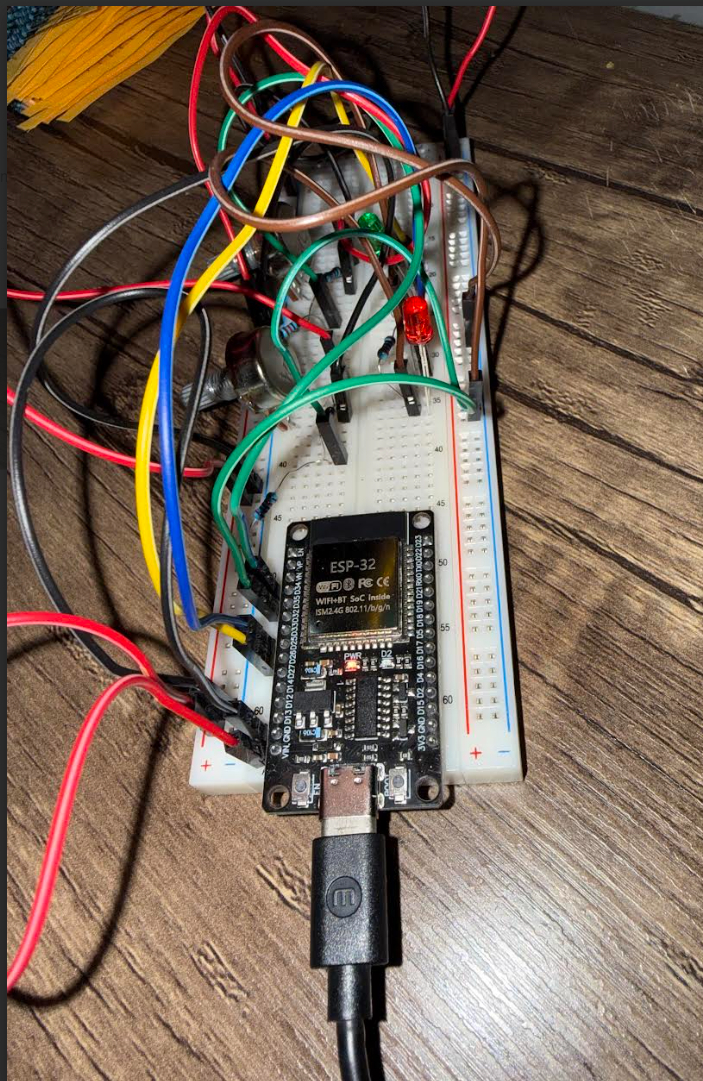
\includegraphics[width=0.75\textwidth]{circuitofisico_1.png} 
		\caption{Vista general del circuito completo armado sobre protoboard, con el LED verde encendido (estado OK, ambos potenciómetros sincronizados).}
	\end{figure}
	
	\begin{figure}[H]
		\centering
		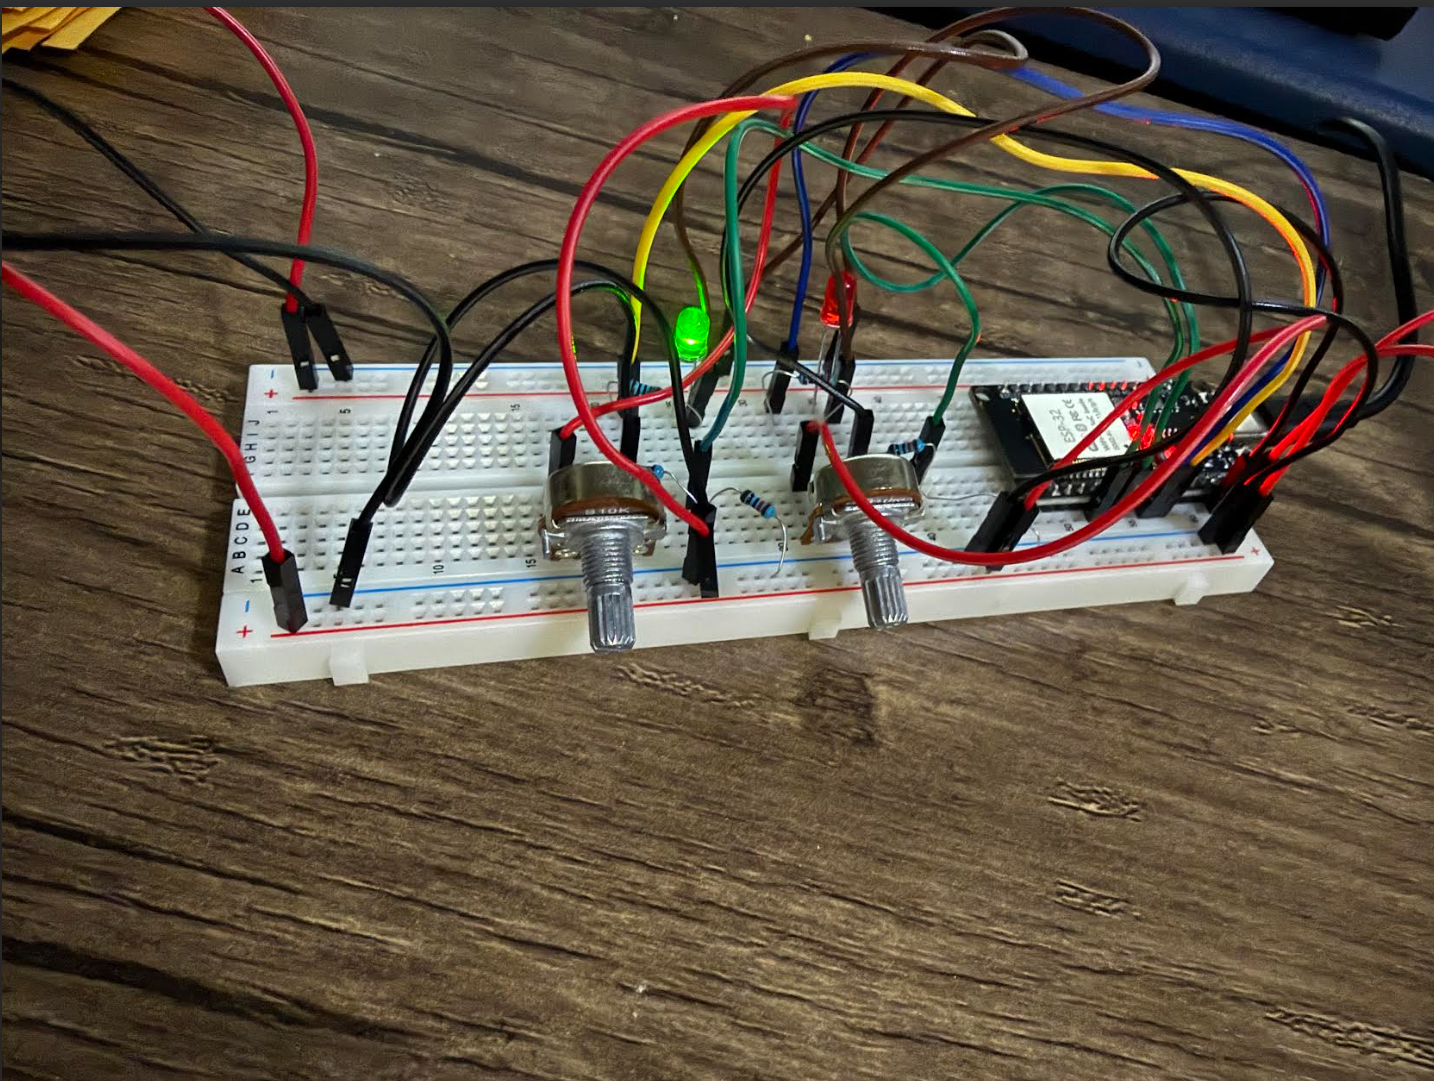
\includegraphics[width=0.75\textwidth]{circuitofisico_2.png} 
		\caption{Vista general del circuito con el LED rojo encendido (estado de falla confirmada, potenciómetros desincronizados).}
	\end{figure}
	
	\begin{figure}[H]
		\centering
		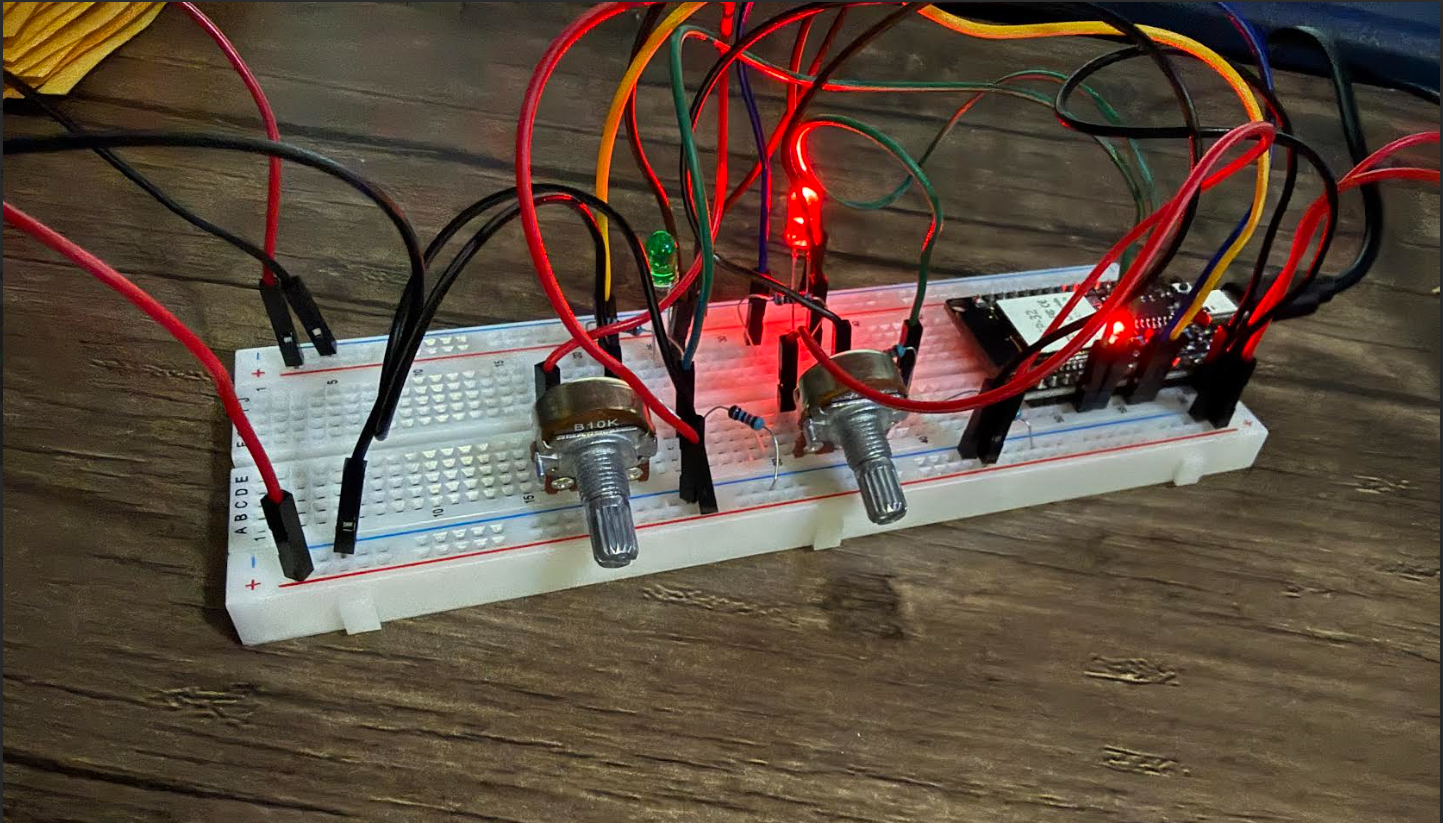
\includegraphics[width=0.75\textwidth]{circuitofisico_3.png} 
		\caption{Vista de detalle del montaje del ESP32 sobre la protoboard, mostrando la conexión de los pines GPIO34, GPIO35, GPIO25, GPIO26 y la alimentación por USB.}
	\end{figure}
	
	% =========================================================================
	% --- SECCIÓN 5: ANÁLISIS DETALLADO DEL CÓDIGO ---
	% =========================================================================
	\section{Análisis Detallado del Código Fuente por Secciones}
	El firmware completo fue desarrollado en C++ sobre el entorno Arduino IDE 2.3.10, dirigido a la placa \texttt{ESP32 Dev Module}. A continuación se documenta cada bloque funcional del código y la justificación técnica detrás de las decisiones tomadas.
	
	\subsection{Definición de Pines}
	\begin{lstlisting}[language=C++]
		const int PIN_SENSOR_1 = 35;   // ADC1_CH7 - Canal A del APPS (post divisor 10k/20k -> ~3.3V)
		const int PIN_SENSOR_2 = 34;   // ADC1_CH6 - Canal B del APPS (post divisor 10k/10k -> ~2.5V)
		const int PIN_LED_ALERTA = 25; // LED rojo: se enciende en falla confirmada
		const int PIN_LED_MOTOR  = 26; // LED verde: encendido = motor habilitado
	\end{lstlisting}
	\textbf{Comentario técnico:} \texttt{GPIO34} y \texttt{GPIO35} fueron elegidos deliberadamente porque pertenecen al conjunto de pines \textit{input-only} del ESP32, es decir, físicamente no cuentan con resistencias de \textit{pull-up/pull-down} internas ni circuitería de salida. Esta característica los hace ideales para lectura analógica pura, pero también los hace especialmente susceptibles a comportarse como entradas flotantes ante cualquier conexión floja — condición que, como se documenta en la Sección 6.3, fue la causa raíz de gran parte del proceso de depuración de este proyecto.
	
	\subsection{Capa de Calibración: la función \texttt{calibrarCanal()}}
	\begin{lstlisting}[language=C++]
		const int ADC_MIN_CH1 = 0;
		const int ADC_MAX_CH1 = 4095;   // corresponde a ~3.3V en canal 1
		const int ADC_MIN_CH2 = 0;
		const int ADC_MAX_CH2 = 3100;   // corresponde a ~2.5V en canal 2 (rango mas chico)
		
		float calibrarCanal(int lecturaCruda, int adcMin, int adcMax) {
			float pct = (float)(lecturaCruda - adcMin) * 100.0 / (float)(adcMax - adcMin);
			if (pct < 0) pct = 0;
			if (pct > 100) pct = 100;
			return pct;
		}
	\end{lstlisting}
	\textbf{Comentario técnico:} la función implementa una interpolación lineal simple (regla de tres) que traduce cualquier lectura cruda al rango 0--100 \%, y aplica un \textbf{recorte (clamping)} en ambos extremos. Este recorte es crítico: sin él, ruido eléctrico que empuje la lectura ligeramente por debajo del mínimo calibrado o por encima del máximo generaría porcentajes negativos o mayores a 100, valores sin sentido físico que podrían propagarse incorrectamente hacia la capa de seguridad y alterar el cálculo de la diferencia entre canales.
	
	El valor de \texttt{ADC\_MAX\_CH2} fue ajustado experimentalmente de 3100 a 2700 durante la fase de pruebas de rango completo (Sección 8), luego de observar que el canal correspondiente no alcanzaba el 100 \% teórico al llevar el potenciómetro a su tope físico. Esta desviación entre el valor teórico de diseño y el valor real medido se explica y documenta en la Sección 6.4.
	
	\subsection{Máquina de Estados de Seguridad}
	\begin{lstlisting}[language=C++]
		const float UMBRAL_PLAUSIBILIDAD_PCT = 10.0;
		const unsigned long TIEMPO_DEBOUNCE_MS = 100;
		
		enum EstadoSeguridad {
			ESTADO_OK,
			ESTADO_FALLA_PENDIENTE,
			ESTADO_FALLA_CONFIRMADA
		};
		
		volatile EstadoSeguridad estadoActual = ESTADO_OK;
		unsigned long tiempoInicioFalla = 0;
		bool fallaEnCurso = false;
	\end{lstlisting}
	\textbf{Comentario técnico:} el sistema se modela como una máquina de estados finitos de tres estados, que resulta el mínimo necesario para representar correctamente el problema:
	\begin{itemize}
		\item \texttt{ESTADO\_OK}: ambos canales coinciden dentro del margen de plausibilidad; el motor permanece habilitado.
		\item \texttt{ESTADO\_FALLA\_PENDIENTE}: existe una discrepancia detectada, pero aún no ha transcurrido el tiempo de \textit{debounce}; el sistema aún no toma una decisión definitiva. Este estado intermedio es indispensable porque distingue entre ruido transitorio (que se autoresuelve) y una falla sostenida real.
		\item \texttt{ESTADO\_FALLA\_CONFIRMADA}: la discrepancia se mantuvo por más de 100 ms de forma continua; el sistema corta el motor de forma inmediata y determinista.
	\end{itemize}
	La variable \texttt{estadoActual} se declara como \texttt{volatile} porque, aunque en esta implementación se modifica únicamente dentro del \texttt{loop()} principal, se mantiene esta calificación como práctica defensiva estándar en sistemas embebidos, dado que su valor está lógicamente ligado al ciclo de muestreo disparado por interrupción de hardware.
	
	\subsection{Adquisición por Interrupción de Hardware (Timer de 1 kHz)}
	\begin{lstlisting}[language=C++]
		hw_timer_t *timerMuestreo = NULL;
		volatile bool banderaMuestreo = false;
		
		void IRAM_ATTR onTimerMuestreo() {
			banderaMuestreo = true;
		}
		
		const int PIN_SENAL_INTERRUPCION = 27;
	\end{lstlisting}
	\textbf{Comentario técnico:} en lugar de leer los sensores directamente dentro del \texttt{loop()} a la velocidad que el procesador tenga disponible, se configuró un temporizador de hardware que dispara una interrupción cada 1000 microsegundos (1 kHz). Esta decisión reproduce una práctica fundamental del diseño de sistemas embebidos de tiempo real: \textbf{un sistema de seguridad no puede depender de que el bucle principal esté libre en el instante exacto en que se necesita un dato}. Si en el futuro se agregara al \texttt{loop()} una tarea que tome varios milisegundos (por ejemplo, comunicación WiFi o escritura en una tarjeta SD), un diseño ingenuo perdería la cadencia de muestreo de los sensores críticos; el uso del temporizador de hardware garantiza que el instante de muestreo permanezca fijo independientemente de la carga del resto del programa.
	
	Es importante notar que la rutina de interrupción (\texttt{onTimerMuestreo}, marcada con \texttt{IRAM\_ATTR} para asegurar que resida en memoria de ejecución rápida) \textbf{no realiza ningún trabajo pesado}: únicamente levanta una bandera booleana (\texttt{banderaMuestreo}). Esta es una regla de oro en la programación de interrupciones: mantenerlas lo más breves posible, delegando el trabajo real (lectura del ADC, operaciones de punto flotante, escritura por puerto serie) al contexto del \texttt{loop()} principal, donde no existe riesgo de bloquear otras interrupciones del sistema ni de generar condiciones de carrera con operaciones más lentas.
	
	El pin \texttt{PIN\_SENAL\_INTERRUPCION} (GPIO27) representa, como se explicó en la Sección 2, la línea física que en un vehículo real se conectaría al sistema de corte de encendido o inyección.
	
	\subsection{\texttt{setup()}: Inicialización del Sistema}
	\begin{lstlisting}[language=C++]
		void setup() {
			Serial.begin(115200);
			pinMode(PIN_LED_ALERTA, OUTPUT);
			pinMode(PIN_LED_MOTOR, OUTPUT);
			pinMode(PIN_SENAL_INTERRUPCION, OUTPUT);
			
			digitalWrite(PIN_LED_ALERTA, LOW);
			digitalWrite(PIN_LED_MOTOR, HIGH);
			digitalWrite(PIN_SENAL_INTERRUPCION, LOW);
			
			analogReadResolution(12);
			
			timerMuestreo = timerBegin(1000000);
			timerAttachInterrupt(timerMuestreo, &onTimerMuestreo);
			timerAlarm(timerMuestreo, 1000, true, 0);
			
			Serial.println("timestamp_ms,ch1_pct,ch2_pct,diferencia_pct,estado");
		}
	\end{lstlisting}
	\textbf{Comentario técnico:} el sistema arranca en un estado seguro y explícito: el LED de alerta apagado, el LED de motor encendido (motor habilitado por defecto) y la señal de interrupción en bajo. La resolución del ADC se fija explícitamente en 12 bits mediante \texttt{analogReadResolution(12)} para garantizar que el rango de lectura (0--4095) coincida exactamente con el asumido en las constantes de calibración de la Sección 5.2, independientemente de la resolución por defecto del núcleo Arduino-ESP32 instalado.
	
	La configuración del temporizador de hardware utiliza la API vigente del núcleo \texttt{arduino-esp32} en su versión 3.x, la cual difiere de versiones anteriores del framework: \texttt{timerBegin()} recibe directamente la frecuencia en Hz a la que corre el contador interno (en este caso, 1 MHz, es decir, cada \textit{tick} del contador equivale a 1 microsegundo), y \texttt{timerAlarm()} sustituye a las funciones separadas \texttt{timerAlarmWrite()} y \texttt{timerAlarmEnable()} de versiones anteriores, configurando en una sola llamada el periodo de disparo (1000 \textit{ticks} = 1000 $\mu$s = 1 ms) y la recarga automática infinita del temporizador. Identificar y adaptar el código a este cambio de API fue uno de los primeros retos técnicos del proyecto, documentado en la Sección 6.
	
	Finalmente, se imprime el encabezado del formato CSV de salida (\texttt{timestamp\_ms,ch1\_pct,ch2\_pct,diferencia\_pct,estado}), que estructura toda la telemetría del sistema en un formato fácilmente auditable y, potencialmente, importable a una hoja de cálculo o a un futuro dashboard de análisis.
	
	\subsection{\texttt{loop()}: Ciclo Principal de Ejecución}
	\begin{lstlisting}[language=C++]
		void loop() {
			if (!banderaMuestreo) return;
			banderaMuestreo = false;
			
			int crudo1 = analogRead(PIN_SENSOR_1);
			int crudo2 = analogRead(PIN_SENSOR_2);
			
			float pct1 = calibrarCanal(crudo1, ADC_MIN_CH1, ADC_MAX_CH1);
			float pct2 = calibrarCanal(crudo2, ADC_MIN_CH2, ADC_MAX_CH2);
			float diferencia = fabs(pct1 - pct2);
			
			bool hayDiscrepancia = (diferencia > UMBRAL_PLAUSIBILIDAD_PCT);
			unsigned long ahora = millis();
			
			if (hayDiscrepancia) {
				if (!fallaEnCurso) {
					fallaEnCurso = true;
					tiempoInicioFalla = ahora;
					estadoActual = ESTADO_FALLA_PENDIENTE;
				} else if (ahora - tiempoInicioFalla > TIEMPO_DEBOUNCE_MS) {
					estadoActual = ESTADO_FALLA_CONFIRMADA;
				}
			} else {
				fallaEnCurso = false;
				estadoActual = ESTADO_OK;
			}
			
			if (estadoActual == ESTADO_FALLA_CONFIRMADA) {
				digitalWrite(PIN_LED_ALERTA, HIGH);
				digitalWrite(PIN_LED_MOTOR, LOW);
				digitalWrite(PIN_SENAL_INTERRUPCION, HIGH);
			} else {
				digitalWrite(PIN_LED_ALERTA, LOW);
				digitalWrite(PIN_LED_MOTOR, HIGH);
				digitalWrite(PIN_SENAL_INTERRUPCION, LOW);
			}
			
			if (ahora - ultimaImpresion >= INTERVALO_IMPRESION_MS) {
				ultimaImpresion = ahora;
				Serial.print(ahora); Serial.print(",");
				Serial.print(pct1, 2); Serial.print(",");
				Serial.print(pct2, 2); Serial.print(",");
				Serial.print(diferencia, 2); Serial.print(",");
				switch (estadoActual) {
					case ESTADO_OK: Serial.println("OK"); break;
					case ESTADO_FALLA_PENDIENTE: Serial.println("PENDIENTE"); break;
					case ESTADO_FALLA_CONFIRMADA: Serial.println("FALLA_CONFIRMADA"); break;
				}
			}
		}
	\end{lstlisting}
	\textbf{Comentario técnico por bloque:}
	\begin{itemize}
		\item \textbf{Guardia de sincronización (\texttt{if (!banderaMuestreo) return;}):} el \texttt{loop()} del ESP32 se ejecuta de forma continua a la máxima velocidad posible del procesador, muy por encima de 1 kHz. Sin esta guardia, el sistema realizaría cientos de miles de lecturas redundantes por segundo, desperdiciando ciclos de CPU y generando ruido innecesario en el puerto serie. Al condicionar todo el trabajo a la bandera levantada por el temporizador de hardware, se garantiza que la lógica de seguridad se ejecute exactamente al ritmo de 1000 veces por segundo, ni más ni menos — la cadencia de muestreo que exige un sistema de seguridad determinista.
		\item \textbf{Adquisición y calibración:} se leen ambos canales y se convierten inmediatamente a porcentaje mediante la función descrita en 5.2, de forma que toda la lógica posterior trabaja exclusivamente en la escala normalizada 0--100 \%, nunca con los valores crudos del ADC.
		\item \textbf{Decisión de plausibilidad:} se calcula la diferencia absoluta entre ambos porcentajes (\texttt{fabs(pct1 - pct2)}) y se compara contra el umbral de 10 \%. El uso de \texttt{fabs()} en lugar de una comparación de magnitudes por separado simplifica la lógica y evita errores de signo, ya que la dirección de la discrepancia (qué canal es mayor que el otro) es irrelevante para la decisión de plausibilidad; lo único relevante es la magnitud de la diferencia.
		\item \textbf{Temporización del debounce:} la variable \texttt{tiempoInicioFalla} únicamente se actualiza en el instante exacto en que comienza una nueva discrepancia (transición de \texttt{false} a \texttt{true} en \texttt{hayDiscrepancia}), no en cada ciclo en el que la discrepancia persiste. Esto es lo que permite medir correctamente cuánto tiempo lleva la falla activa de forma continua, en lugar de reiniciar el conteo en cada muestra.
		\item \textbf{Recuperación automática (\texttt{else \{ fallaEnCurso = false; estadoActual = ESTADO\_OK; \}}):} en el instante en que ambos canales vuelven a coincidir dentro del margen de plausibilidad, el sistema regresa automáticamente al estado \texttt{OK}, sin requerir intervención externa ni reinicio manual del microcontrolador. Esta es una decisión de diseño documentada explícitamente en la Sección 8, adoptada tras validar experimentalmente que el sistema exhibe este comportamiento, y es coherente con la filosofía de un sistema de plausibilidad que reacciona en tiempo real a la condición eléctrica presente, sin mantener memoria de fallas pasadas ya resueltas.
		\item \textbf{Actuación desacoplada del muestreo de impresión:} las líneas que controlan los LEDs y la señal de interrupción se ejecutan en cada ciclo de 1 ms, independientemente de si ese ciclo corresponde o no a un instante de impresión por puerto serie. Esto garantiza que el tiempo de reacción físico del sistema (LEDs, señal de corte) sea siempre de 1 ms, mientras que la salida legible por humanos en el Monitor Serie se limita a una impresión cada 200 ms mediante la comparación \texttt{ahora - ultimaImpresion >= INTERVALO\_IMPRESION\_MS}. Esta separación evita saturar el puerto serie —a 115200 baudios, imprimir en cada ciclo de 1 ms generaría un volumen de datos que el propio proceso de impresión no podría desalojar a tiempo, terminando por ralentizar el bucle de seguridad— y es un patrón estándar en sistemas embebidos: \textit{bucle de control rápido, telemetría lenta}.
	\end{itemize}
	
	% =========================================================================
	% --- SECCIÓN 6: DETECCIÓN Y CORRECCIÓN DE ERRORES ---
	% =========================================================================
	\section{Detección y Corrección de Errores Durante el Desarrollo}
	Durante el ciclo de desarrollo se presentaron varias fallas, tanto de software como de hardware, cuya identificación y corrección se documentan a continuación siguiendo un orden cronológico, ya que cada una condicionó la solución de la siguiente.
	
	\subsection{Fallo de Comunicación Serial en Simulación (Wokwi)}
	Antes de construir el circuito físico, se elaboró una simulación completa en la plataforma Wokwi, incluyendo el esquemático con el ESP32, ambos potenciómetros, las resistencias de los divisores y los LEDs. La simulación corrió correctamente a nivel de tiempos de ejecución (uso de CPU estable, temporizador activo), pero el Monitor Serie de la plataforma nunca mostró salida alguna, pese a que el código era idéntico al que posteriormente funcionó en hardware real. Ante la imposibilidad de diagnosticar esta limitación de la herramienta de simulación en el tiempo disponible, se optó por priorizar la validación directamente sobre hardware físico, documentando este punto como una limitación conocida de la fase de simulación y no del diseño del sistema.
	
	\subsection{Lecturas ADC Fijas en Cero (Circuito Abierto)}
	La primera versión del circuito físico, con ambos potenciómetros, sus divisores de voltaje y los LEDs ya conectados, mostraba en el Monitor Serie una salida constante de \texttt{0.00,0.00,0.00,OK} sin importar la posición de las perillas. Para descartar variables, se aisló el problema mediante un \textit{sketch} de diagnóstico mínimo que solo imprimía las lecturas crudas de \texttt{analogRead(34)} y \texttt{analogRead(35)}, sin ninguna capa de calibración ni de seguridad de por medio. El resultado confirmó que ambos canales permanecían en cero de forma persistente incluso al mover físicamente los potenciómetros, lo cual descartaba un error de software y apuntaba a una \textbf{discontinuidad eléctrica} en la ruta señal-divisor-GPIO: en ese momento, la hipótesis más probable era que la alimentación de 5 V no estaba llegando correctamente a las patas VCC de los potenciómetros.
	
	\subsection{Oscilación Errática por Conexiones Flojas (Falsos Contactos)}
	Al reconstruir el circuito de forma simplificada —un solo potenciómetro, sin resistencias de divisor, alimentado directamente a 3.3 V y conectado directo al GPIO correspondiente— se observó un segundo fenómeno: las lecturas ya no se quedaban fijas en cero, pero \textbf{oscilaban erráticamente entre 0 y el valor máximo (4095) sin que nadie tocara el potenciómetro}, incluso con la perilla completamente inmóvil. Este patrón es la firma característica de una \textbf{entrada flotante intermitente}: los pines \texttt{GPIO34} y \texttt{GPIO35} del ESP32, al ser pines de solo entrada sin resistencias internas de \textit{pull-up/pull-down} (como se documentó en la Sección 5.1), son extremadamente sensibles al ruido electromagnético ambiental (EMI) y a la capacitancia parásita cuando la conexión física no es sólida.
	
	La estrategia de diagnóstico aplicada fue de \textbf{aislamiento progresivo}: se desconectó todo excepto el canal bajo prueba, y se presionó manualmente, uno por uno, cada punto de contacto de la cadena señal $\rightarrow$ protoboard $\rightarrow$ GPIO, observando en tiempo real el efecto sobre el Monitor Serie. Este método permitió confirmar que el problema era, en efecto, mecánico y no eléctrico de fondo: la simple presión manual sobre los cables estabilizaba las lecturas de forma instantánea y correlacionada.
	
	\textbf{Solución aplicada:} fijación de cada conexión crítica (pata del potenciómetro–jumper, jumper–protoboard, jumper–GPIO) mediante cinta adhesiva, eliminando el juego mecánico de los cables. Tras esta intervención, las lecturas mostraron una progresión suave, monotónica y libre de saltos al girar la perilla, confirmando la resolución del problema. Esta misma disciplina de fijación se replicó sistemáticamente en cada conexión añadida posteriormente (divisores de resistencias, LEDs), evitando la reaparición del fenómeno en el circuito completo.
	
	\subsection{Desviación de Calibración por Tolerancia de Resistencias Reales}
	Una vez estabilizado el hardware, la prueba de rango completo (girar cada potenciómetro hasta su tope físico) reveló que el Canal 2 (\texttt{GPIO34}) no alcanzaba el 100 \% calibrado, estabilizándose alrededor del 90 \%, mientras que el Canal 1 (\texttt{GPIO35}) sí alcanzaba correctamente el 100 \%. Esto no representa una falla de hardware, sino una consecuencia esperada de trabajar con \textbf{componentes reales}: las resistencias comerciales tienen una tolerancia (típicamente $\pm$5 \% o mayor en resistencias de baja precisión) respecto a su valor nominal, por lo que el divisor de 10 k$\Omega$/10 k$\Omega$ del Canal 2 no produce en la práctica exactamente 2.5 V de tope, sino un valor ligeramente distinto al valor teórico usado inicialmente para definir la constante \texttt{ADC\_MAX\_CH2}.
	
	\textbf{Solución aplicada:} se recalibró empíricamente la constante \texttt{ADC\_MAX\_CH2}, llevando el potenciómetro a su tope físico real y registrando el valor crudo del ADC obtenido en ese punto, ajustando la constante de 3100 a 2700. Tras la corrección, la prueba de rango completo mostró que ambos canales alcanzan de forma limpia y consistente 0.00 \% y 100.00 \% en sus extremos. Este ajuste ilustra en la práctica el valor de la separación entre la capa de calibración y la capa de seguridad descrita en la Sección 3: corregir una desviación de hardware real requirió modificar una única constante, sin alterar ninguna línea de la lógica de plausibilidad, del \textit{debounce} ni de la máquina de estados.
	
	% =========================================================================
	% --- SECCIÓN 7: EVOLUCIÓN DEL CIRCUITO ---
	% =========================================================================
	\section{Evolución del Circuito Físico: De la Primera Versión al As-Built}
	El circuito experimentó una evolución significativa entre su primer intento de armado y la versión final validada:
	\begin{itemize}
		\item \textbf{Versión inicial (teórica):} divisores de voltaje planeados con el potenciómetro de mayor rango (10 k$\Omega$/20 k$\Omega$) asignado a \texttt{GPIO34} y el de menor rango (10 k$\Omega$/10 k$\Omega$) asignado a \texttt{GPIO35}, alimentación directa a 5 V, sin verificación experimental de conexiones.
		\item \textbf{Versión intermedia (diagnóstico):} simplificación deliberada del circuito a un solo canal, sin resistencias de divisor, alimentado a 3.3 V directo, utilizada exclusivamente como banco de pruebas para aislar el problema de conexiones flojas descrito en la Sección 6.3, antes de reintroducir la complejidad completa del circuito.
		\item \textbf{Versión final (As-Built):} ambos potenciómetros alimentados en 5 V (\texttt{VIN}) con sus respectivos divisores resistivos, con la asignación de pines corregida en software (\texttt{PIN\_SENSOR\_1 = 35}, \texttt{PIN\_SENSOR\_2 = 34}) para reflejar la disposición física real del cableado, todas las conexiones críticas fijadas mecánicamente, y la constante \texttt{ADC\_MAX\_CH2} recalibrada a 2700 con base en mediciones reales.
	\end{itemize}
	Esta evolución documentada — de un diseño teórico, pasando por una etapa de diagnóstico simplificado, hasta un As-Built corregido con datos empíricos — refleja el mismo principio de ingeniería iterativa aplicado en el desarrollo de software: el diseño en papel es un punto de partida necesario, pero la validación experimental sistemática es la que determina la implementación final confiable.
	
	% =========================================================================
	% --- SECCIÓN 8: PROTOCOLO DE PRUEBAS ---
	% =========================================================================
	\section{Protocolo de Pruebas de Validación y Resultados Obtenidos}
	Una vez estabilizado el hardware y recalibrado el sistema, se ejecutó un protocolo formal de seis pruebas funcionales, cuyos resultados se resumen en la siguiente tabla:
	
	\begin{table}[H]
		\centering
		\footnotesize
		\begin{tabular}{c p{3.5cm} p{4cm} p{3.5cm} p{3.5cm}}
			\toprule
			\textbf{\#} & \textbf{Prueba} & \textbf{Procedimiento} & \textbf{Resultado esperado} & \textbf{Resultado obtenido} \\
			\midrule
			1 & Movimiento sincronizado (caso normal) & Mover ambos potenciómetros al mismo tiempo y velocidad & LED verde permanece encendido; estado \texttt{OK} constante & Confirmado \\
			\addlinespace
			2 & Falla por desincronización & Mover un solo potenciómetro, dejando el otro fijo, con diferencia mayor al 10 \% & LED rojo se enciende y permanece encendido; estado \texttt{FALLA\_CONFIRMADA} & Confirmado \\
			\addlinespace
			3 & Recuperación tras falla & Tras una falla confirmada, resincronizar ambos potenciómetros & El sistema regresa automáticamente a \texttt{ESTADO\_OK} sin reinicio manual & Confirmado — el sistema recupera de forma automática \\
			\addlinespace
			4 & Filtro de \textit{debounce} & Desincronizar los potenciómetros por menos de 100 ms & El estado transita a \texttt{PENDIENTE} y regresa a \texttt{OK} sin llegar a \texttt{FALLA\_CONFIRMADA} & Confirmado — únicamente se activa \texttt{FALLA\_CONFIRMADA} cuando la discrepancia supera los 100 ms; discrepancias breves quedan en \texttt{PENDIENTE} y se autoresuelven \\
			\addlinespace
			5 & Rango completo de calibración & Llevar cada potenciómetro a sus topes físicos (0 \% y 100 \%) & Ambos canales alcanzan 0.00 \% y 100.00 \% de forma limpia & Confirmado tras el ajuste de \texttt{ADC\_MAX\_CH2} de 3100 a 2700 (ver Sección 6.4) \\
			\addlinespace
			6 & Consistencia del formato CSV & Registro continuo del Monitor Serie durante operación normal & Formato \texttt{timestamp\_ms, ch1\_pct, ch2\_pct, diferencia\_pct, estado} legible y sin errores de formato & Confirmado \\
			\bottomrule
		\end{tabular}
	\end{table}
	
	\begin{figure}[H]
		\centering
		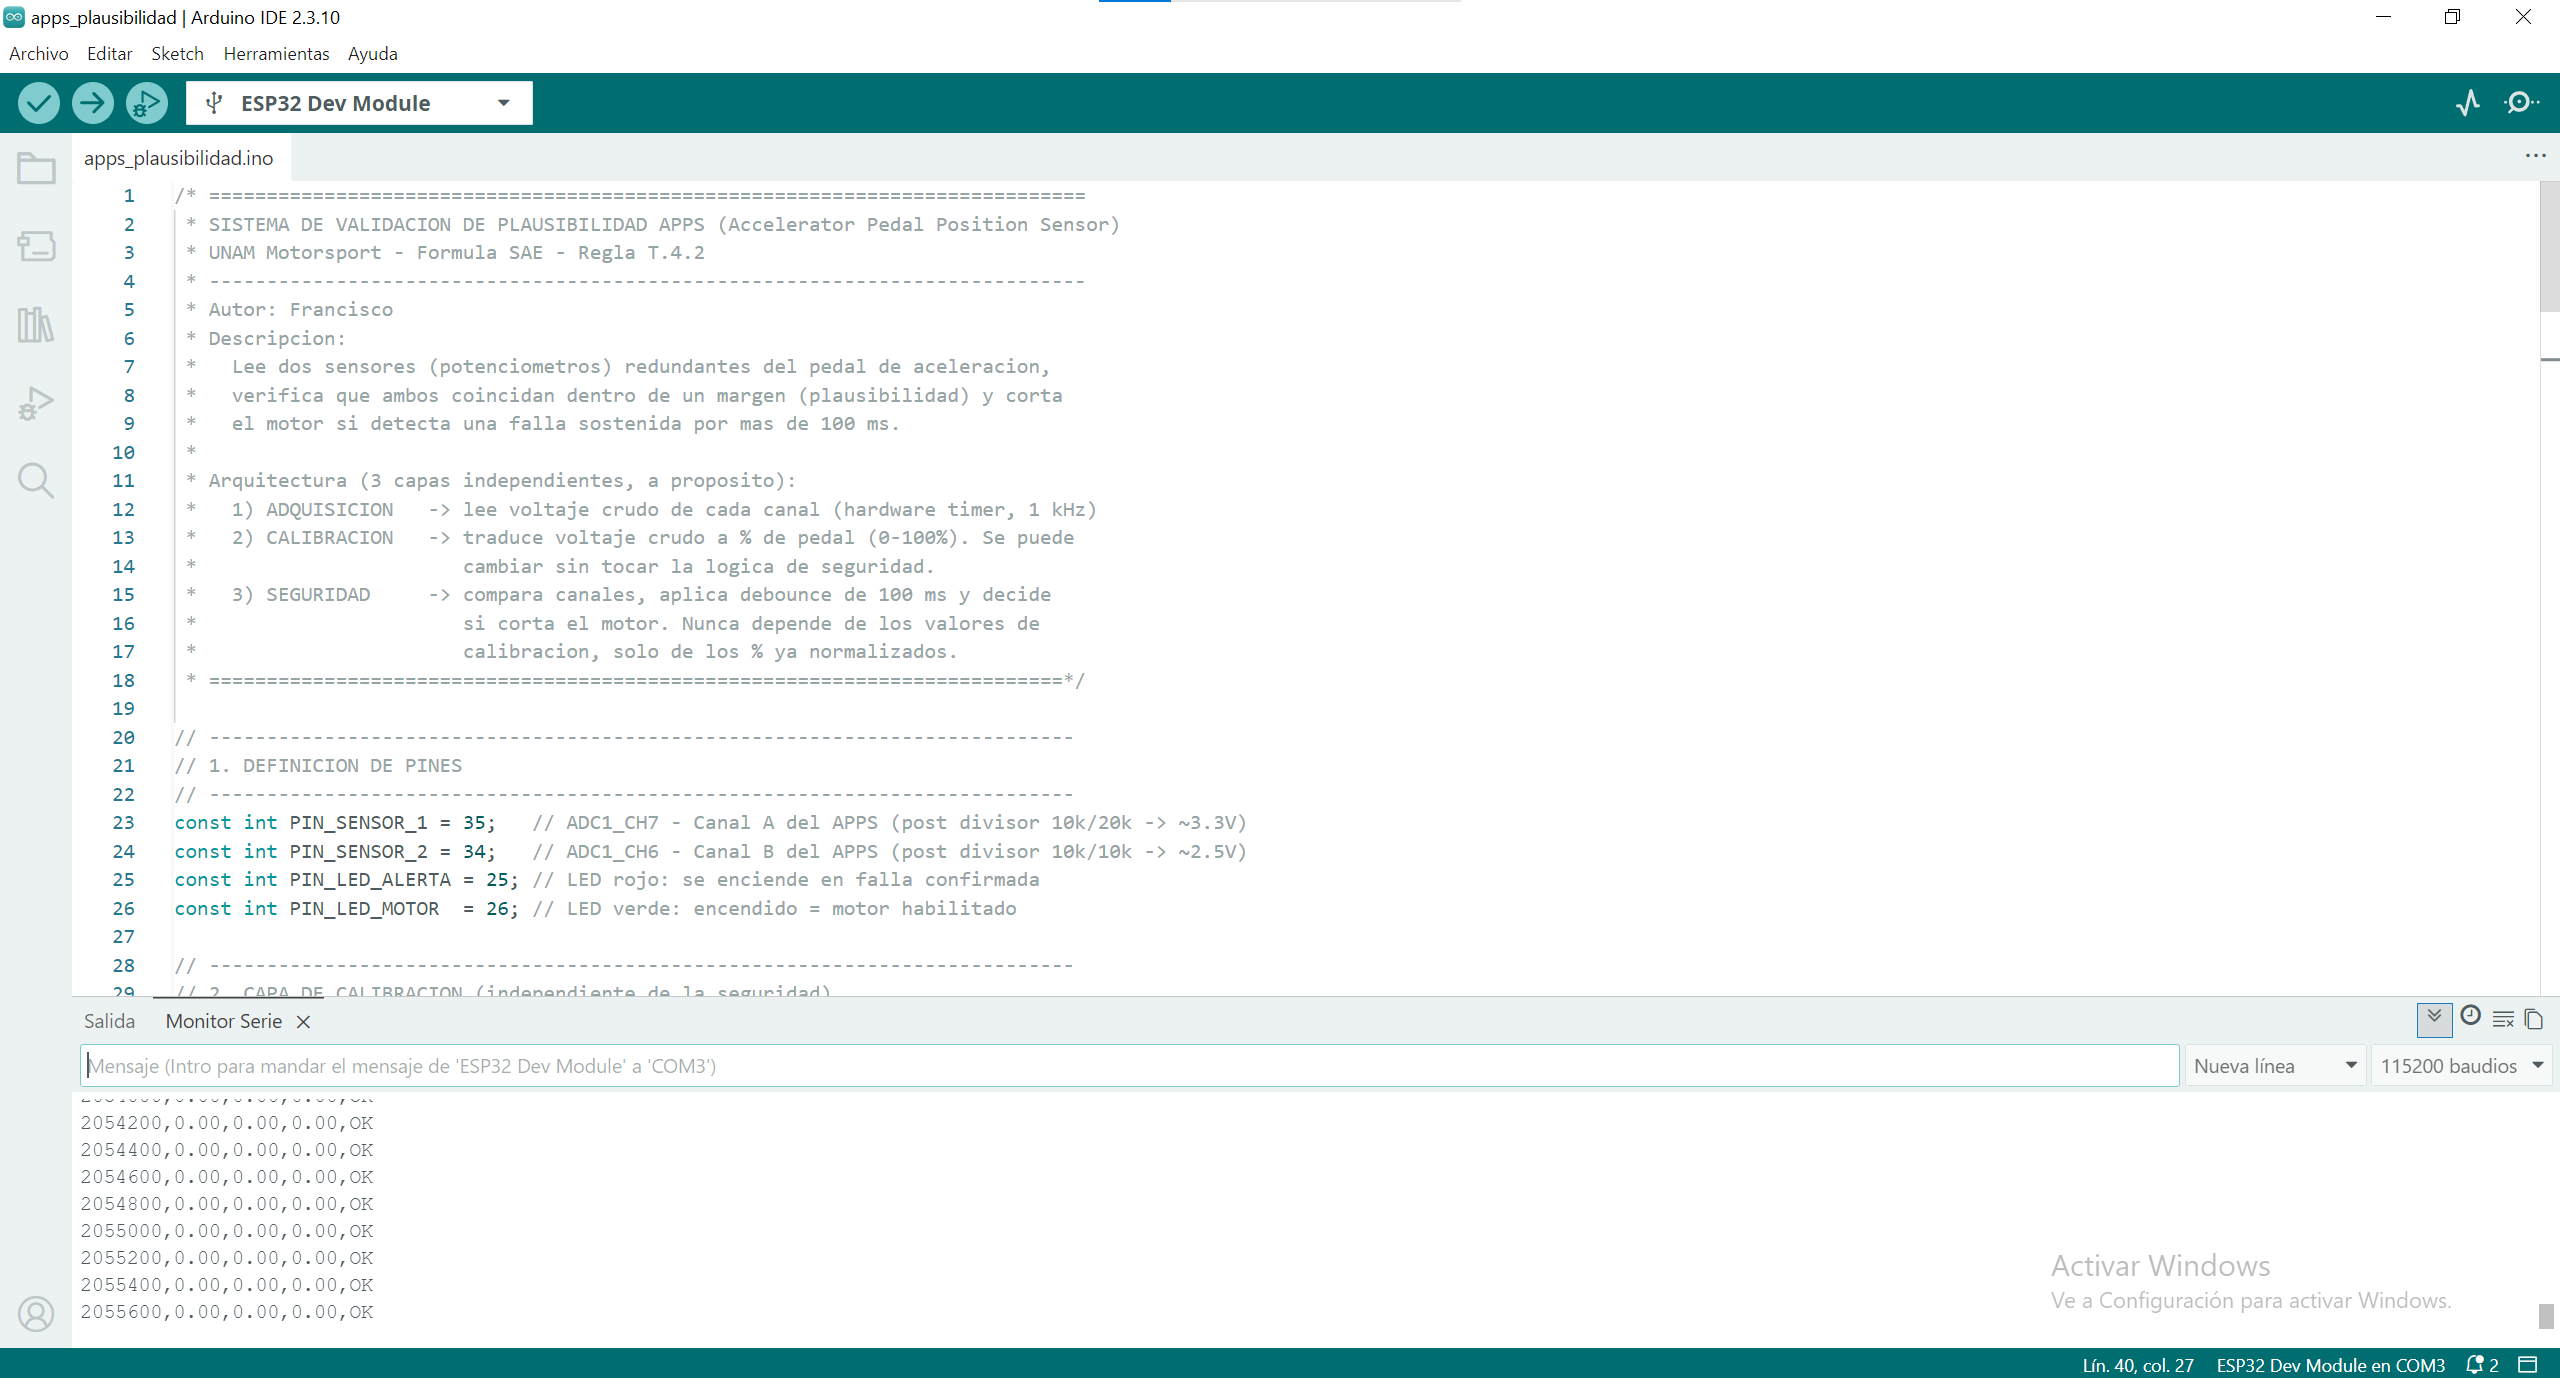
\includegraphics[width=0.75\textwidth]{apps_1.png} 
		\caption{Captura de Monitor Serie mostrando el ciclo completo de recuperación automática: transición OK $\rightarrow$ PENDIENTE $\rightarrow$ FALLA\_CONFIRMADA $\rightarrow$ OK.}
	\end{figure}
	
	\begin{figure}[H]
		\centering
		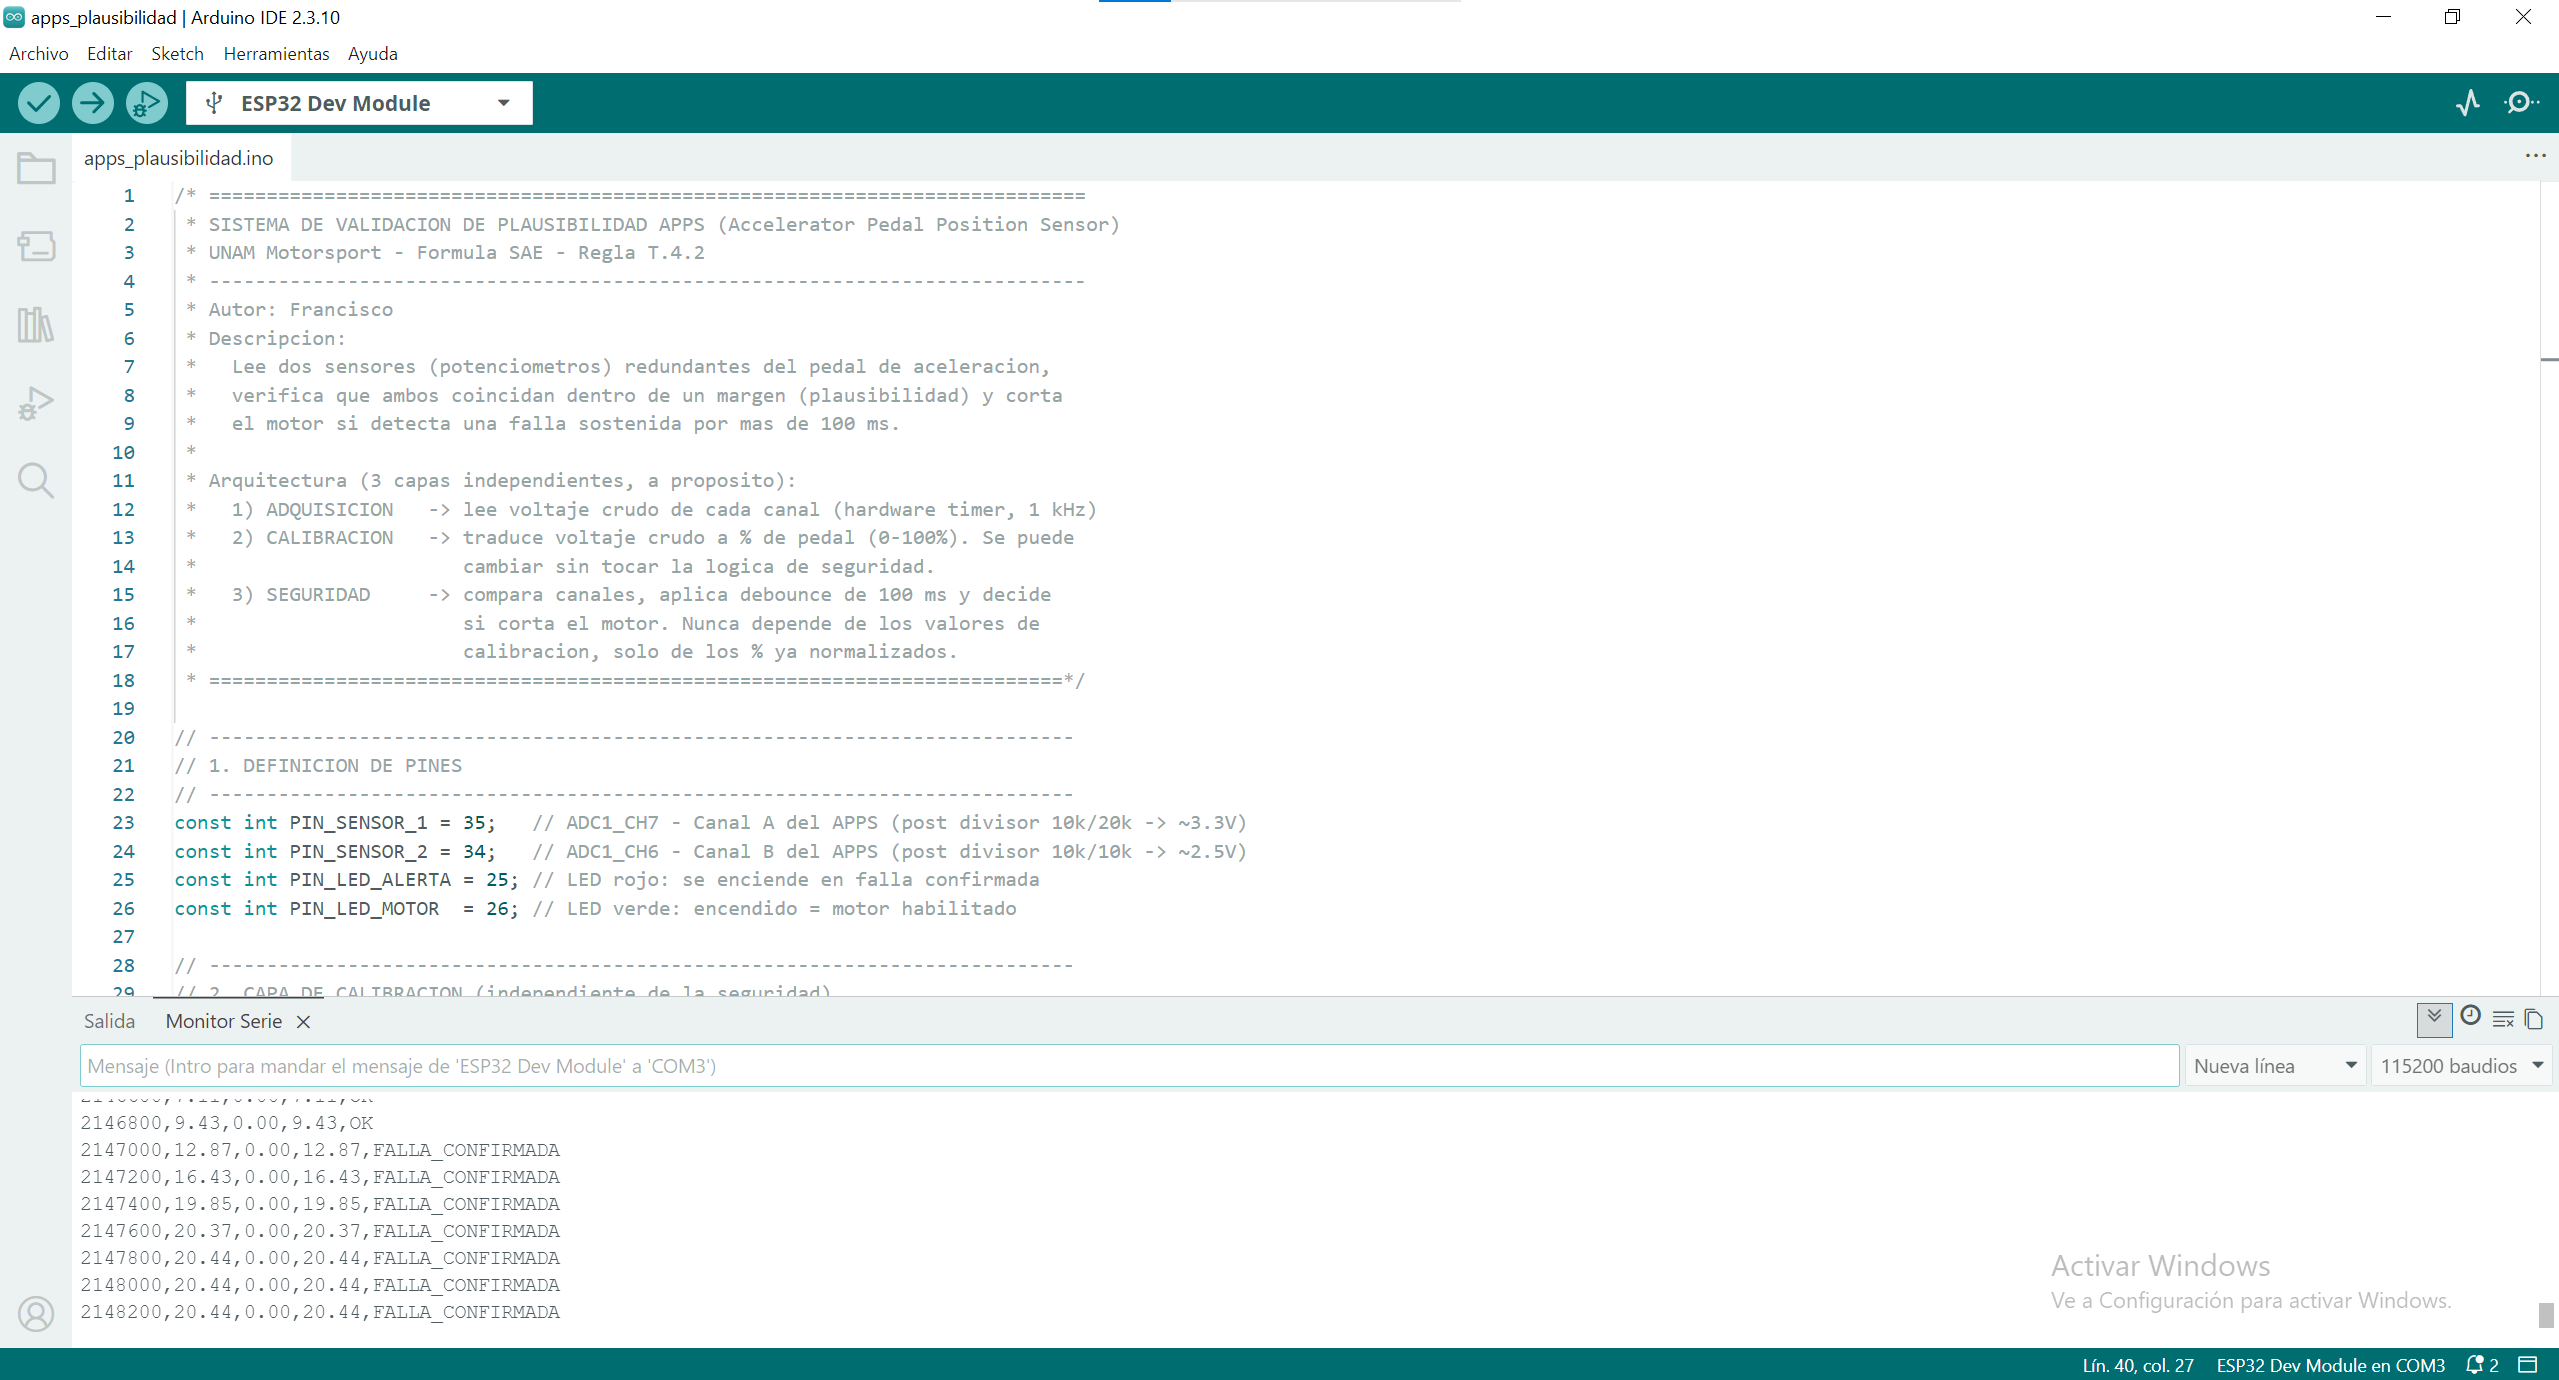
\includegraphics[width=0.75\textwidth]{apps_2.png} 
		\caption{Captura de Monitor Serie de la prueba de rango completo, mostrando la transición limpia hasta 100.00 \% en ambos canales y su estabilidad sostenida en el tope.}
	\end{figure}
	
	\begin{figure}[H]
		\centering
		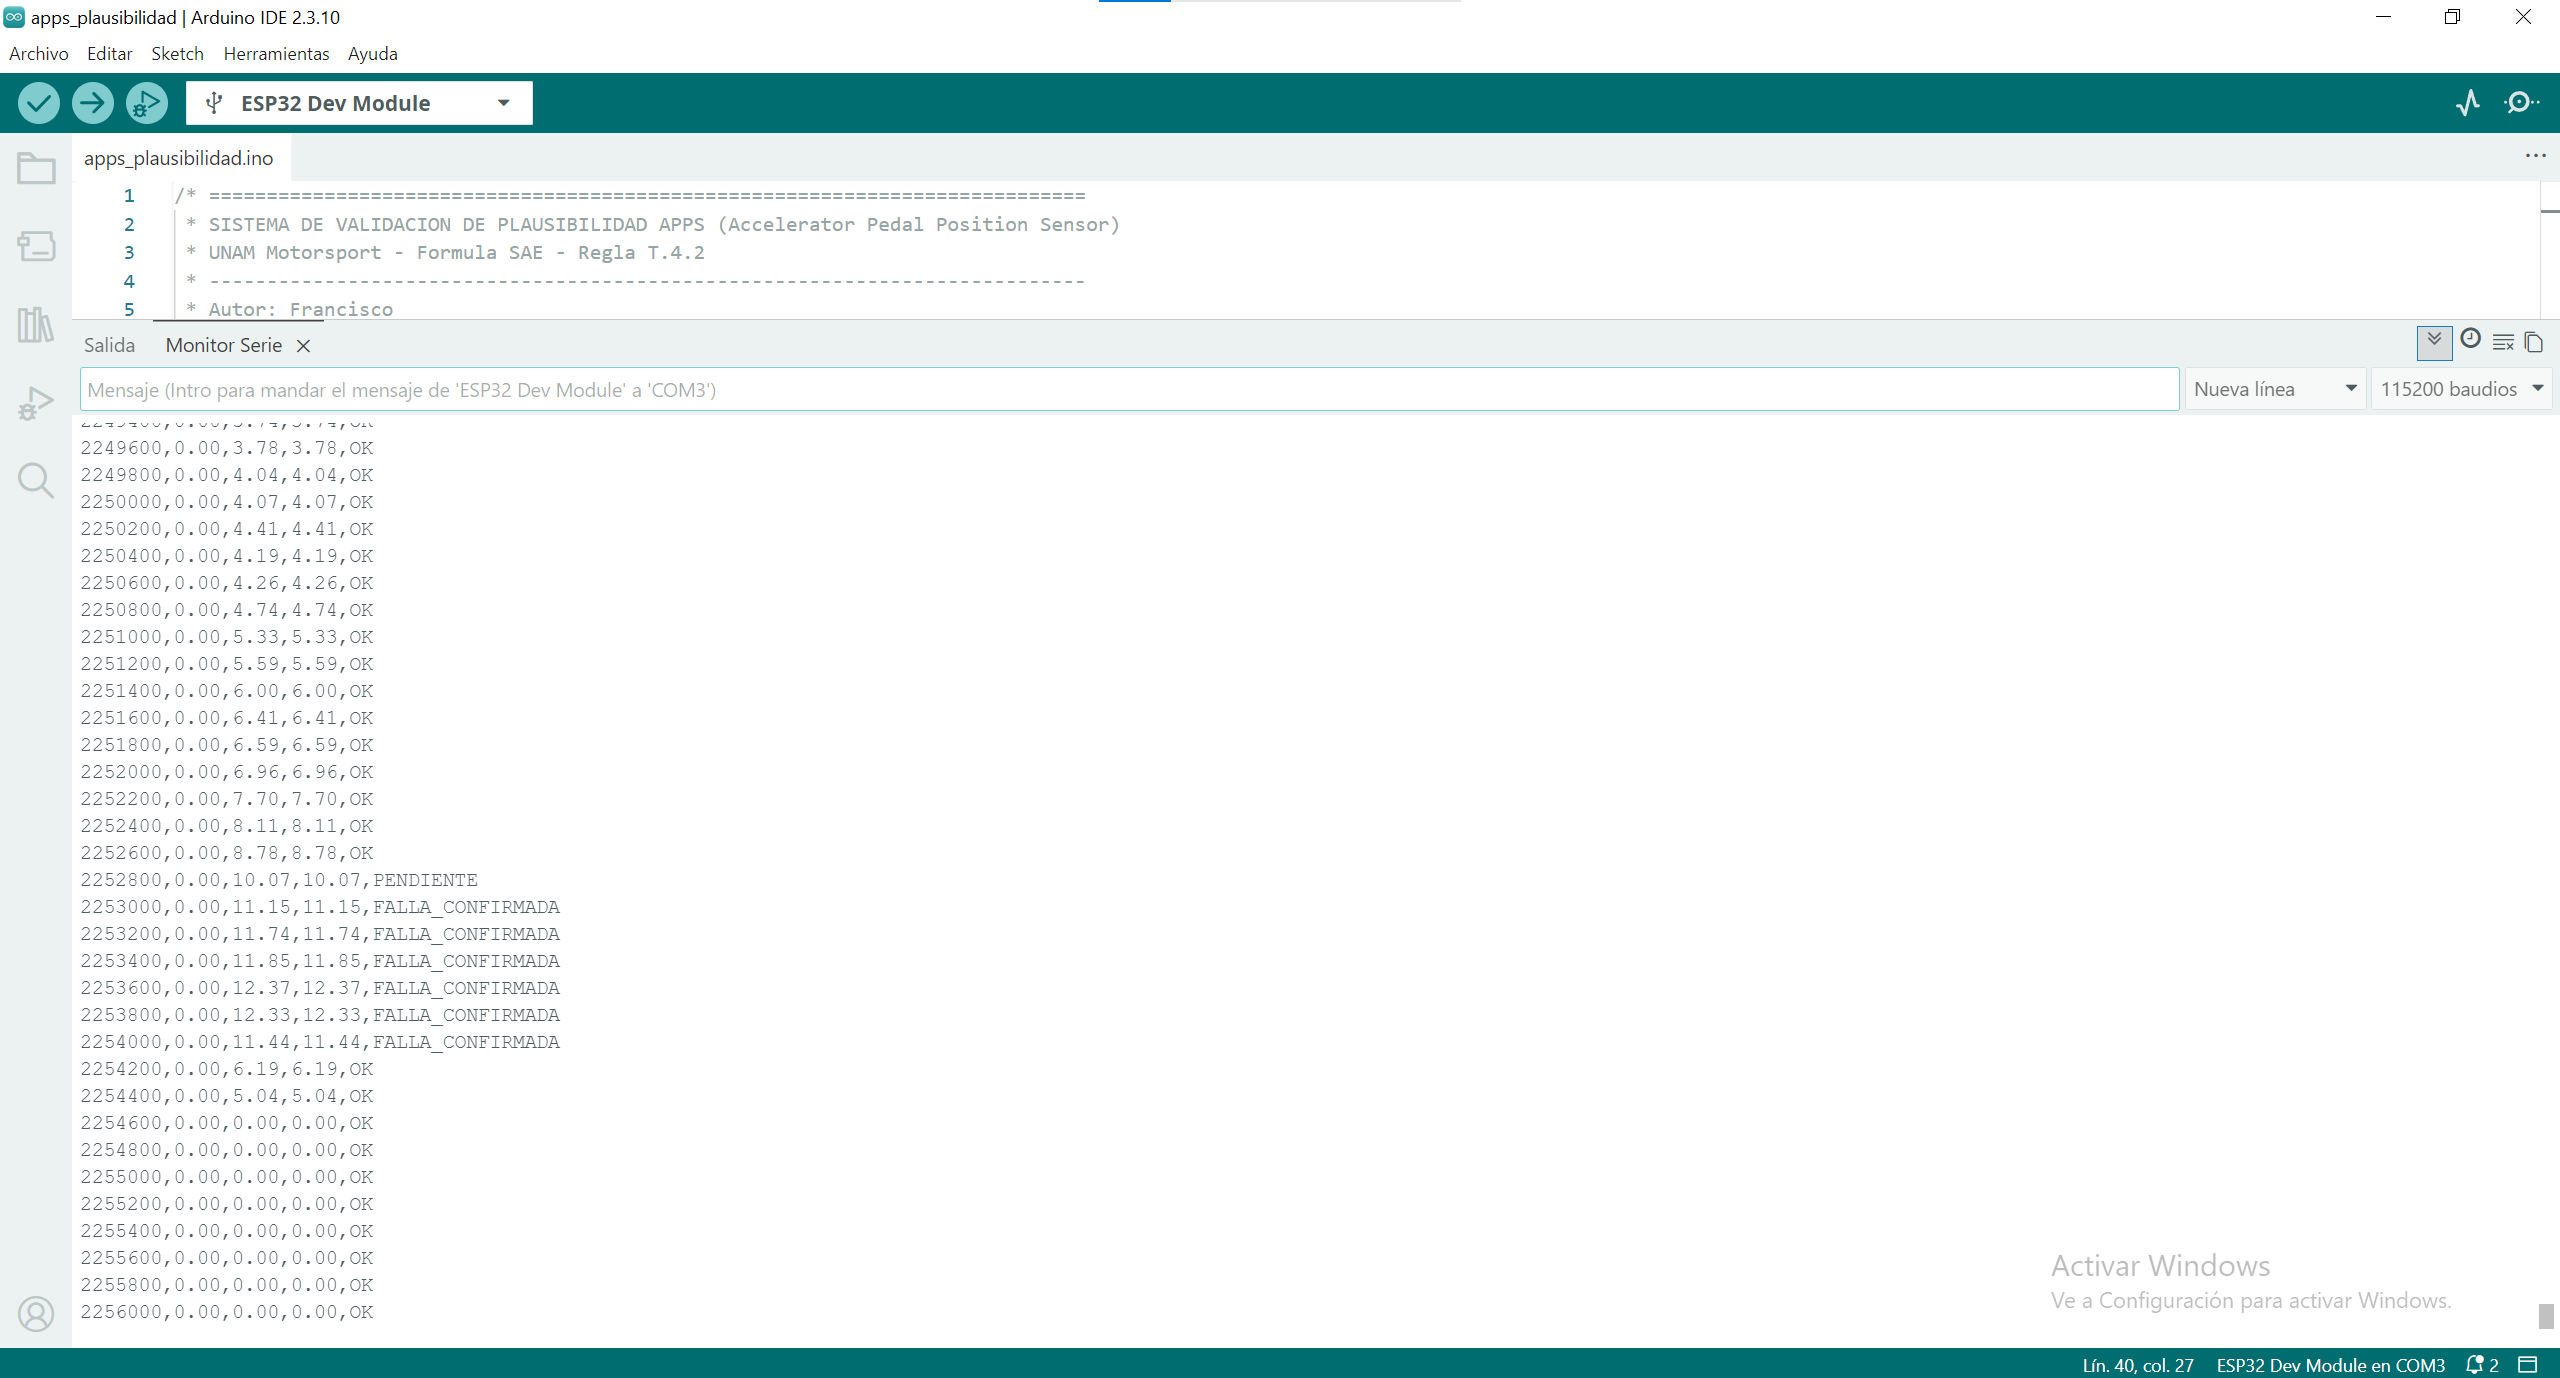
\includegraphics[width=0.75\textwidth]{apps_3.png} 
		\caption{Captura de Monitor Serie de la prueba de debounce/falla sostenida, mostrando el encabezado del código junto con una secuencia de \texttt{FALLA\_CONFIRMADA} mantenida en el tiempo.}
	\end{figure}
	
	\begin{figure}[H]
		\centering
		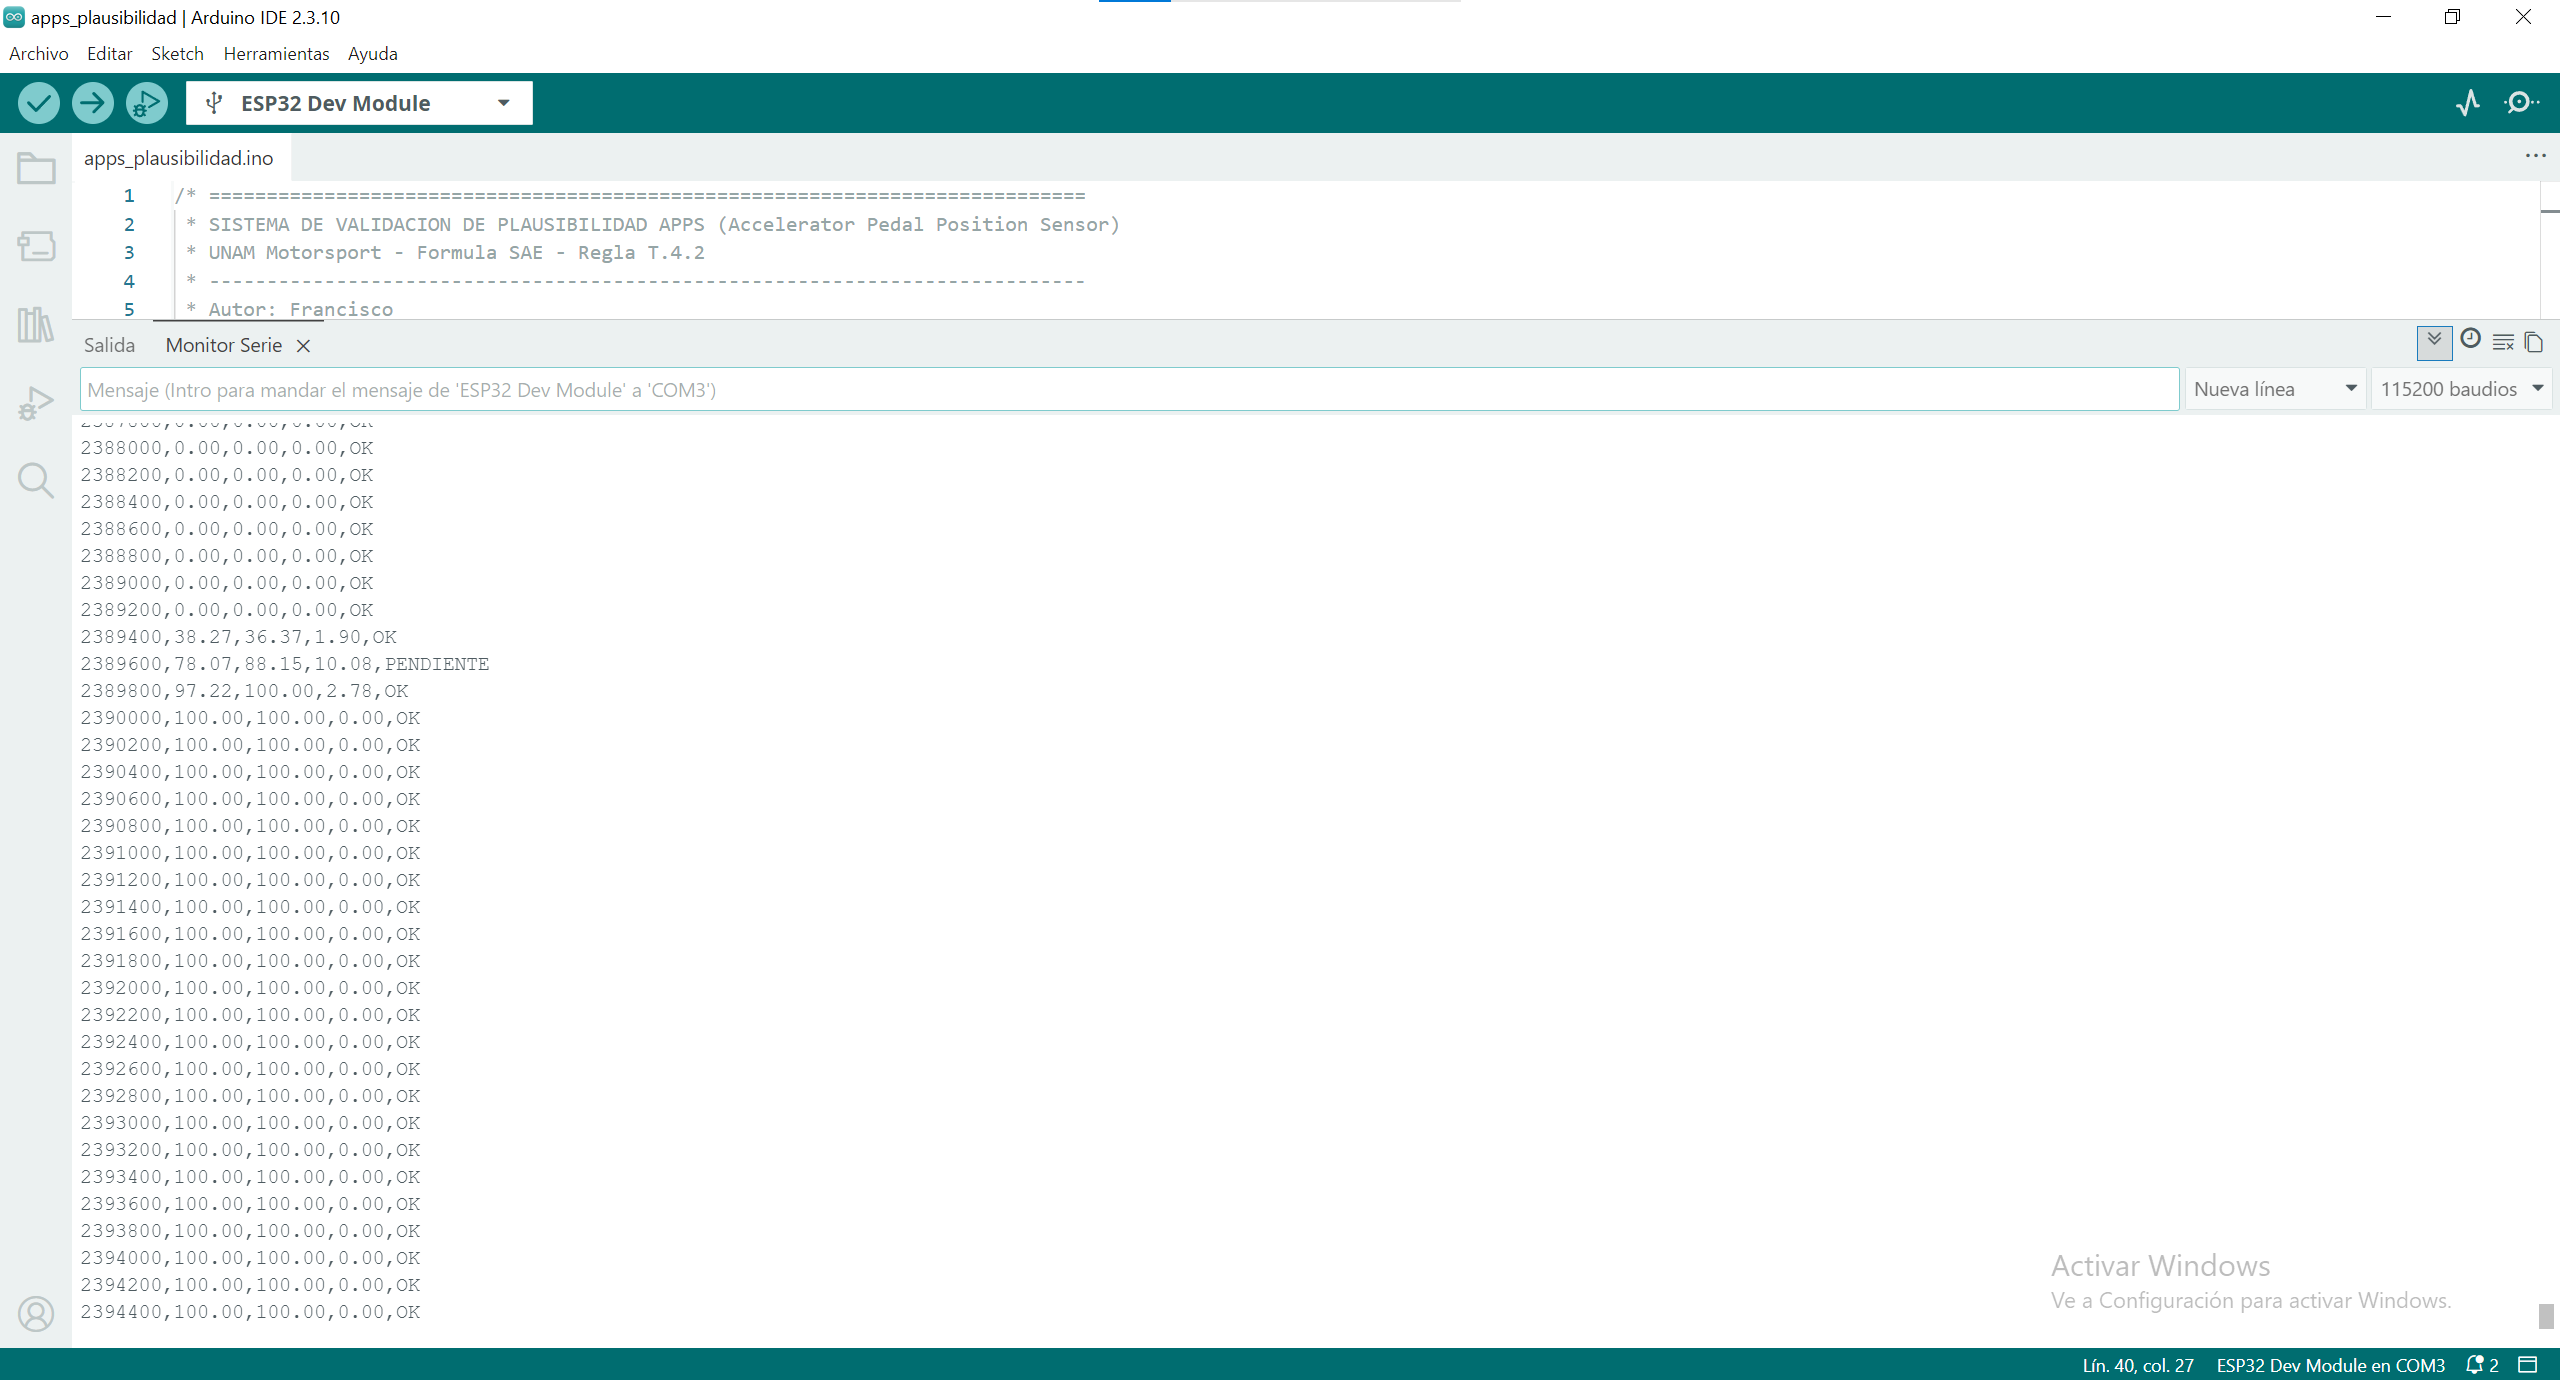
\includegraphics[width=0.75\textwidth]{apps_4.png} 
		\caption{Captura de Monitor Serie en estado estable \texttt{OK}, evidenciando la limpieza del formato CSV durante operación normal.}
	\end{figure}
	
	Las decisiones de diseño validadas por estas pruebas —en particular, la recuperación automática del estado \texttt{OK} sin intervención manual, y la tolerancia del sistema a discrepancias breves inferiores a 100 ms— constituyen respuestas explícitas a preguntas de diseño que un sistema de seguridad crítico debe resolver de forma consciente, y se documentan aquí como decisiones deliberadas y verificadas, no como comportamientos accidentales del código.
	
	% =========================================================================
	% --- SECCIÓN 9: NOTA METODOLÓGICA ---
	% =========================================================================
	\section{Nota Metodológica: Primera Experiencia con Sistemas Embebidos y Uso de Herramientas de IA}
	Es pertinente señalar que esta actividad representó mi primera experiencia programando un microcontrolador y trabajando con sistemas embebidos en general, incluyendo el manejo de interrupciones de hardware, temporizadores, conversión analógico-digital y el diseño de circuitos con divisores de voltaje sobre protoboard. Dado este contexto, el desarrollo del proyecto se apoyó de forma activa en dos fuentes complementarias de conocimiento:
	
	\begin{enumerate}
		\item \textbf{Documentación oficial}, consultada de forma directa para fundamentar cada decisión técnica del proyecto: la documentación de Espressif Systems sobre el hardware del ESP32 (características del ADC, pines de solo entrada, especificaciones eléctricas), la documentación oficial del framework Arduino-ESP32 para el manejo de temporizadores de hardware, y el reglamento técnico de Formula SAE para fundamentar los requisitos normativos del sistema de plausibilidad del APPS.
		\item \textbf{Asistencia de Claude (Anthropic)}, utilizada como herramienta de apoyo para: investigar y contrastar el comportamiento esperado del hardware del ESP32 frente a los síntomas observados durante la depuración (por ejemplo, para identificar que la oscilación errática de las lecturas ADC descrita en la Sección 6.3 correspondía a un patrón característico de entradas flotantes en pines \textit{input-only}); guiar paso a paso el proceso de diagnóstico eléctrico del circuito físico ante la ausencia de un multímetro funcional disponible; revisar y corregir fragmentos específicos del código, incluyendo la adaptación a la API vigente de temporizadores de hardware del núcleo \texttt{arduino-esp32} 3.x; y estructurar la metodología de pruebas de validación final documentada en la Sección 8.
	\end{enumerate}
	
	Documento este proceso de forma explícita porque considero que forma parte íntegra del criterio de evaluación de la actividad: el sistema final no solo funciona correctamente, sino que refleja un proceso genuino de aprendizaje autodirigido, combinando fuentes primarias de documentación técnica oficial con herramientas de asistencia inteligente utilizadas de forma responsable, como apoyo al razonamiento propio y no como sustituto de este.
	
	% =========================================================================
	% --- SECCIÓN 10: CONCLUSIONES ---
	% =========================================================================
	\section{Conclusiones}
	El desarrollo de este sistema de validación de plausibilidad para el APPS permitió aplicar, en un prototipo físico funcional, los principios normativos que rigen la seguridad del sistema de aceleración en un vehículo de Formula SAE bajo la regla T.4.2. La arquitectura de tres capas independientes —adquisición, calibración y seguridad— demostró ser una decisión de diseño acertada: permitió aislar y corregir errores de hardware real (conexiones flojas, tolerancia de componentes) modificando exclusivamente la capa correspondiente, sin comprometer en ningún momento la integridad de la lógica de seguridad.
	
	El proceso de depuración documentado en este reporte —desde lecturas fijas en cero, pasando por oscilaciones erráticas de entradas flotantes, hasta la recalibración empírica del rango de un canal— fue, en sí mismo, tan formativo como el diseño original del sistema, y evidencia que la validación experimental sistemática es indispensable en el desarrollo de sistemas embebidos, incluso cuando el diseño teórico de partida es correcto. El protocolo final de seis pruebas confirmó que el sistema cumple de forma consistente con los tres comportamientos exigidos por un sistema de plausibilidad real: tolerancia a operación normal sincronizada, corte confiable ante discrepancia sostenida, y filtrado efectivo de ruido transitorio mediante el mecanismo de \textit{debounce}.
	
	% =========================================================================
	% --- BIBLIOGRAFÍA ---
	% =========================================================================
	\newpage
	\renewcommand{\refname}{Bibliografía}
	\begin{thebibliography}{9}
		
		\bibitem{espressif_datasheet} 
		Espressif Systems. (2024). \textit{ESP32 Series Datasheet} (Versión 4.6). Espressif Systems. Recuperado de \url{https://www.espressif.com/sites/default/files/documentation/esp32_datasheet_en.pdf}
		
		\bibitem{espressif_manual} 
		Espressif Systems. (2024). \textit{ESP32 Technical Reference Manual} (Versión 5.4). Espressif Systems. Recuperado de \url{https://www.espressif.com/sites/default/files/documentation/esp32_technical_reference_manual_en.pdf}
		
		\bibitem{espressif_timer} 
		Espressif Systems. (s.f.). \textit{Arduino-ESP32: Timer API}. Arduino-ESP32 Documentation. Recuperado de \url{https://docs.espressif.com/projects/arduino-esp32/en/latest/api/timer.html}
		
		\bibitem{arduino_analog} 
		Arduino. (s.f.). \textit{analogRead() — Language Reference}. Arduino Reference. Recuperado de \url{https://www.arduino.cc/reference/en/language/functions/analog-io/analogread/}
		
		\bibitem{sae_rules} 
		SAE International. (2024). \textit{2024 Formula SAE Rules} (Sección T.4: Accelerator Pedal Position Sensor / Cortes de Potencia). SAE International. Recuperado de \url{https://www.fsaeonline.com/cdsweb/gen/DocumentResources.aspx}
		
	\end{thebibliography}
	
\end{document}